\subsubsection{Environmental Microbiology - Microbial Habitats}
\index{Boetius, Antje}
%\section{Research on microbial habitats in marine ecosystems (Antje Boetius)}

\paragraph{Research Team}
%
The labs and offices of the Microbial Habitat group lead by Prof. Boetius are at the Max Planck Institute for Marine Microbiology in Bremen. The group consists of 6 scientists and post docs, 9 PhD students, 5 master students and 10 technicians. More information is available at http://www.mpi-bremen.de/en/Habitat$\_$group.html.\\

The microbial habitat describes the physical location and type of environment in which a population of microorganisms lives. Hence, this research group, situated at the Max Planck Institute for Marine Microbiology in Bremen, studies the physical, chemical, geological hydrological and biological characteristics of diverse microbial habitats in the ocean. Microbial populations occupy certain niches in the marine environment, which are defined by a variety of biotic and abiotic factors. The goal of our research on ``microbial habitats'' is to understand niche formation and to investigate regulatory mechanisms for the occurrence and distribution of microbial populations. This requires the development of a variety of molecular and \textit{in situ} techniques, as well as experimental strategies to quantify the nature and variability of the habitat and its inhabiting populations on different temporal and spatial scales.

\paragraph{Highlights}
%
In 2006 we carried out several research cruises studying physical, biological and chemical characteristics of microbial habitats of fluid, gas and mud seeps at continental margins. Together with the observation of physico-chemical characteristics we have analyzed the biogeochemical and ecological consequences of seepage, as well as the associated microbial diversity and population dynamics. Our research is accompanied by several advances in marine technologies, to resolve the spatial and temporal dynamics of microbial habitats \textit{in situ}. Fieldwork has taken us to coastal sites in the North and Baltic Seas, and to deep sea expeditions in the Gulf of Mexico, the Northwest and South Pacific, the Barents Sea, and Eastern Mediterranean. We have obtained the first \textit{in situ} sediment oxygen consumption, sulfide fluxes, methane turnover rates and nutrient exchange rates in cold seep sediments. Important findings include the distribution and metabolic properties of methanotrophic microorganisms at two highly active seeps, one of which represents a natural CO2 lake in the deep sea, and another one which is one of the most active submarine mud volcanoes. This research has been carried out in the framework of a BMBF/DFG Geotechnologien project on methanotrophic microorganisms in deep water gas hydrate bearing systems, studying their molecular diversity, microbiology and biogeochemistry (project MUMM II, coordination A. Boetius); as well as within the work package ``Anoxic microbial habitats'' belonging to the 6th FP EU Integrated Project HERMES ``Hotspot ecosystem research on margins of European Seas''. A variety of anoxic habitats can be found on continental margins that harbor a great diversity of bacteria and archaea. Such microbial ecosystems are found in deep subsurface sediments, at fluid escape structures, below hydrocarbon seeps, above gas hydrates and at mud volcanoes, pockmarks and other cold seep systems. The aim of our future research on these ecosystems which are often associated with fluid flow and gas hydrates is to identify the key microbes providing sources and sinks of carbon by molecular tools, to know their biodiversity, and to understand the energy budget and ecosystem structure of these systems resembling life on early earth. Our integrative research approach will combine molecular biology, microbiology, geochemistry, geology, geophysics, oceanography and modeling of geochemical, and microbiological processes.
%Figure \ref{Boetius_2006_fig}


\begin{figure}[ht]
  \begin{center}
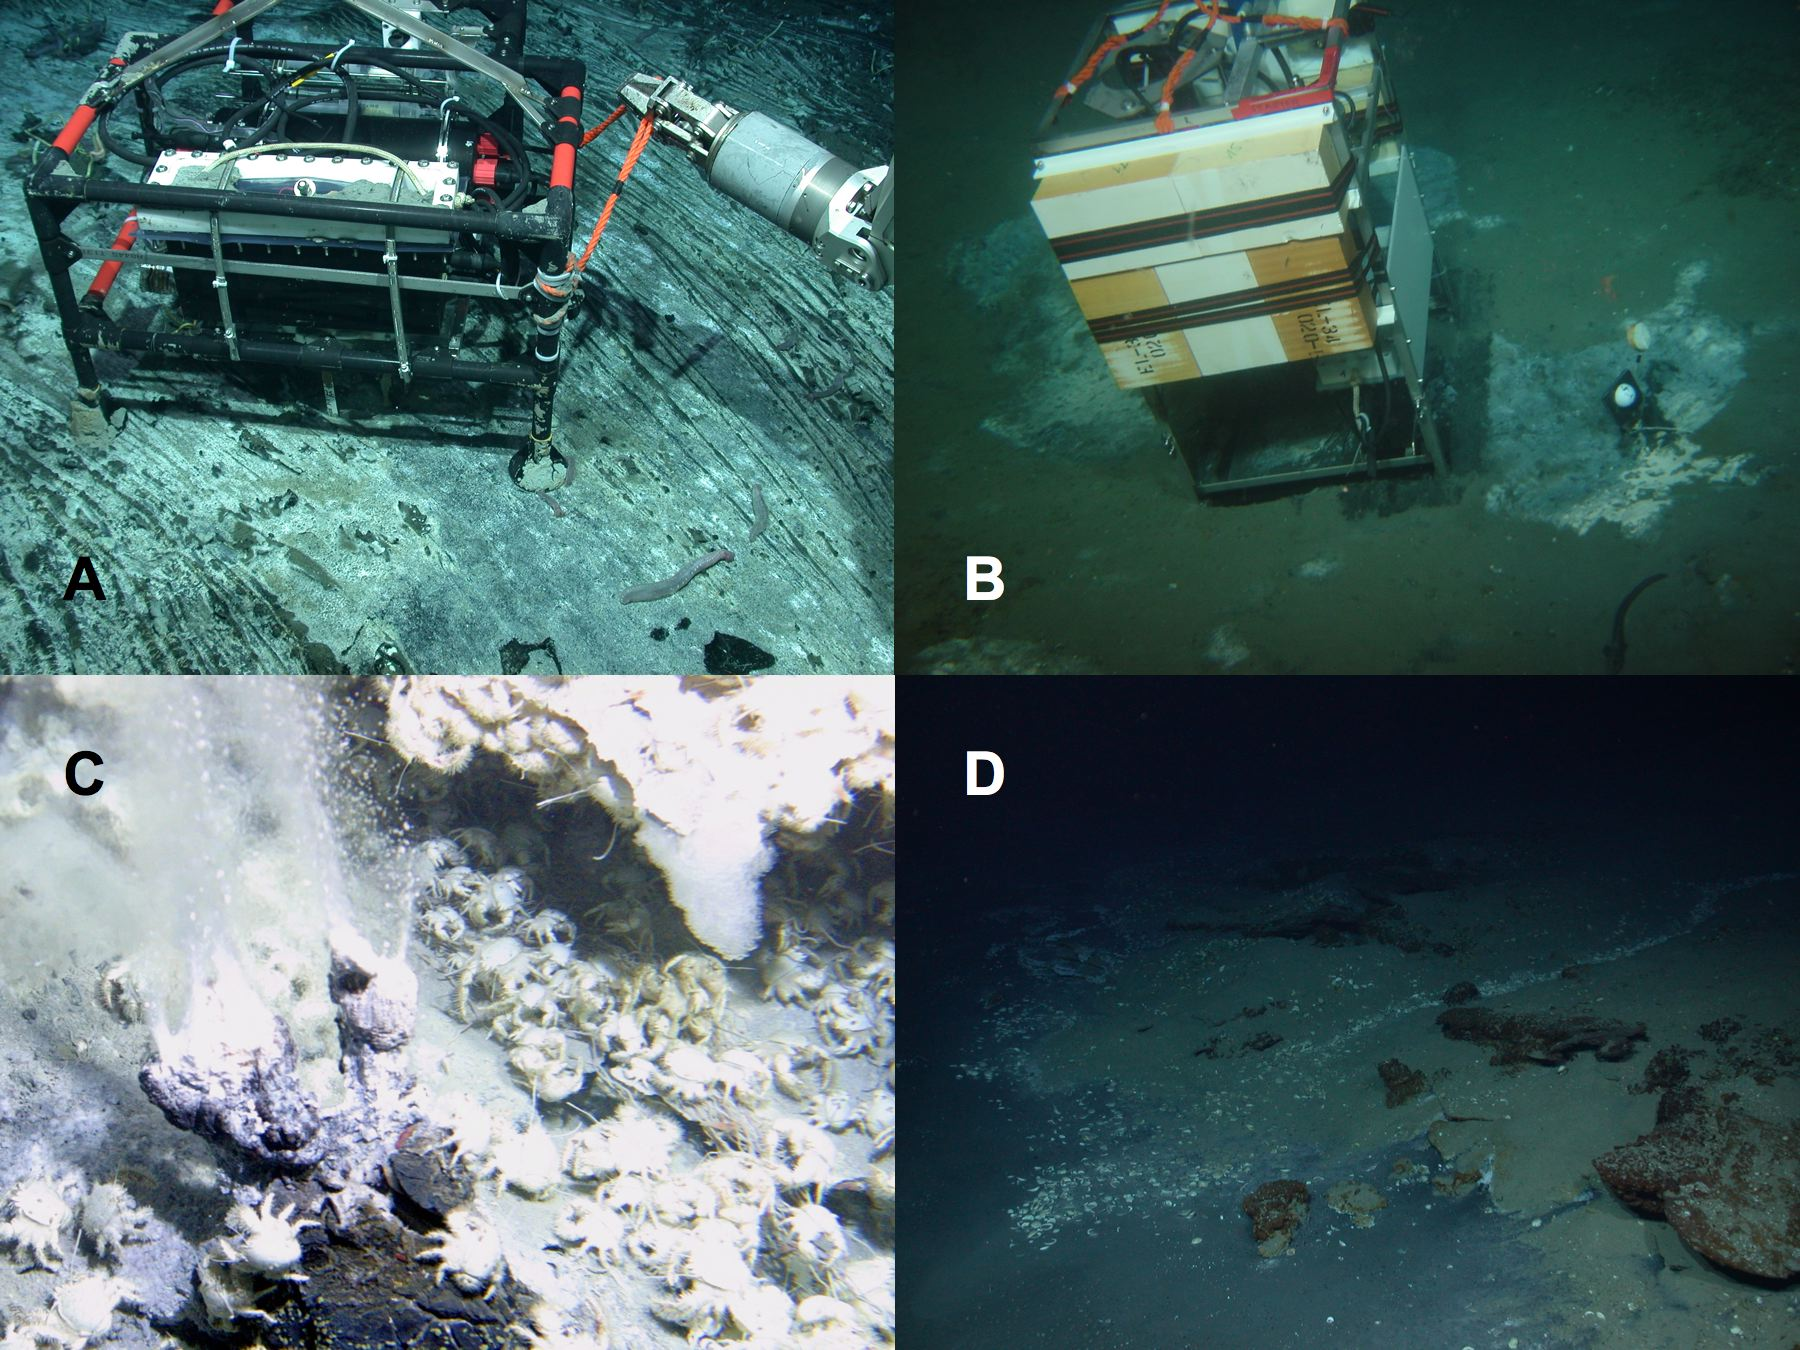
\includegraphics[width=\hsize]{Boetius/Boetius_2006_fig.jpg}
    \mycaption{Microbial habitats at cold seeps of continental margins.  (A) Measuring oxygen flux on a microbial mat covering a natural asphalt flow in the Gulf of Mexico (3000m). (B) Measuring sulfide fluxes on a microbial mat of the Haakon Mosby Mud Volcano (Barents Sea); Niemann and Treude et al., Nature, 2006 (C) Life at a natural $\mbox{CO}_{\mbox{{\footnotesize 2}}}$ lake (Okinawa Trough); Inagaki et al., PNAS, 2006 (D)  Sulfidic subsurface sediments flowing from a mud volcano of the deep Nile fan (Eastern Mediterranean).}
    \label{Boetius_2006_fig}
  \end{center}
\end{figure}

Furthermore we have focused on microbial diversity and community structures in coastal sands. In recent years, an increasing number of microbial studies have addressed the role of space and time in generating diversity patterns in microorganisms. However, the relative contribution of spatio-temporal effects vs. variation of physical and chemical parameters on diversity is still poorly understood, especially in marine sediments. The coastal zones of the ocean are highly productive ecosystems, which despite their relatively small area, play a large role on the global cycles of carbon and nitrogen. Biodiversity and species composition are changing at an increasing rate due to coastal development, eutrophication, pollution, exploitation, species introduction and possibly global warming. Hence, a thorough understanding of the transport processes, material flows and biodiversity within these ecosystems is needed. We are studying a subtidal coastal area of the North Sea island Sylt, where long-term studies ($>$50 yrs) are available.  Special features of this coastal ecosystem are the substantial temperature changes (0-22�C) throughout the year, the impact of storms, the strong pelagic phytoplankton bloom in spring, and the benthic diatom bloom in spring and autumn.



\myparagraph{Collaborations}
%
Bremen Area Collaborations:
\begin{enumerate}
\item {\sl AWI}\\ Dr. M. Klages, Prof. M. Schl�ter \\ Helmholtz Virtual Institute for Marine Technologies, Deep water ecosystems
\item {\sl Jacobs University Bremen} \\ Prof. M. Ullrich \\ Marine Microbiology
\end{enumerate}
National \& International Collaborations:
\begin{enumerate}
\item {\sl IFREMER, France } \\ Dr. K. Olu, Dr. J.P. Foucher\\ Investigation of cold seep ecosystems on continental margins
\item {\sl University of Aveiro, Portugal} \\ Prof. L. Pinheiro\\ Mud volcanoes of the Gulf of Cadiz; DAAD student exchange
\item {\sl University of Georgia, Atlanta, USA} \\ Prof. S. Joye \\ Cold seeps of the Gulf of Mexico, microbiology of oily sediments
\item {\sl University of North Carolina, Chapel Hill, USA} \\ Prof. C. Arnosti \\ Degradation of organic matter in coastal sediments
\item {\sl University of Sunderland, UK} \\ Dr. A. Judd \\ Active gas seeps of the North Sea
\item {\sl University of Hawaii, Hawaii, USA} \\ Prof. C. Smith \\ Microbiology and Biogeochemistry of Sunken Whales and Woods
\item {\sl University of Paris 6, France} \\ Dr. Francoise Gaill \\ Microbiology and Biogeochemistry of Sunken Woods (GDRE DIWOOD)
\item {\sl Pennsylvania State University, Philadelphia, USA} \\ Prof. C. Fisher \\ Microbial ecology and biogeochemistry of cold seep communities in the Gulf of Mexico
\item {\sl IfM-GEOMAR, Kiel}\\ Prof. E. Suess, Dr. O. Pfannkuche, Dr. P. Linke, Prof. K. Wallmann \\ Gas hydrate systems
\end{enumerate}

\goodbreak
\paragraph{Grants at the Max Planck Institute for Marine Microbiology}
% list the running grants in 2006, if none have been received, please delete this
% subsection.
\nobreak
\begin{enumerate}
\item 2007-2012 Graduate School of the Excellence Initiative ``GLOMAR''
\item 2006-2010 ESF EUROCORES EuroDiversity ``MicroSystems''
\item 2006-2009 CNRS GDRE DIWOOD Collaboration Univ Pierre et Marie Curie, CNRS
\item 2005-2009 EU 6th FP IP HERMES ``Hotspot ecosystem research on margins of Europe's seas''
\item 2005-2009 DFG research center ``ocean margins'' E Fluid and gas seepage at continental margins
\item 2005-2008 BMBF project MUMM ``Microbial turnover of methane above marine gas hydrate''
\item 2005-2007 6th FP EU project STREP ``EXOCET  Extreme ecosystem studies in the deep Ocean: technological developments''
\item 2003-2006 ESF project ``MEDIFLUX - Fluid flow, fluid chemistry and cold seep biology in active and passive margin settings of the eastern Mediterranean Sea''
\end{enumerate}

\nocite{Boetius1,Boetius2,Boetius3,Boetius4,Boetius5,Boetius6,Boetius7}
